\paragraph{Error control.}
In the first design the two forecasters have equal expected interval
scores, so $\Dbar_t=0$. Forecaster $A$ issues $[-k_A\sigma_t,k_A\sigma_t]$, where $k_A$ is
$0.85$ times the $(1-\alpha/2)$-quantile of the errors, and $B$ issues the
wider $[-k_B\sigma_t,k_B\sigma_t]$, with $k_B$ chosen so that both expected
scores coincide. Outcomes are standard Gaussian with $\sigma_t=1$, or
$y_t=\sigma_t\varepsilon_t$ with Student-$t_3$ errors and a lognormal scale
$\sigma_t$
(log-standard deviation $0.5$) known to both forecasters. For each
$\alpha\in\{0.2,0.1,0.05,0.02,0.01\}$ we run 1000 replications of length
4000 and evaluate the procedures at $T\in\{250,1000,4000\}$.
Table~\ref{tab:null} and Figure~\ref{fig:dm} report the results.

The empirical-Bernstein (EB) sequence never excluded zero in the
Student-$t$ design and did so in at most 0.1\% of replications in the
Gaussian design, and the Hoeffding sequence never did; the tuned
sequence of Section~\ref{sec:cs}, tuned on the first 10\% of each horizon
$T$ and evaluated at $T$, erred in at most 0.3\%. The asymptotic sequence of
\citet{waudbysmith2024time} is set to be tightest at $t=500$ and
monitored from round 31, since its variance estimate is degenerate in the
first rounds. It excluded zero at some round
in 2.5--4.8\% of Gaussian replications at $\alpha=0.2$, but in 58--60\% at
$\alpha=0.01$, and in 72--75\% at $\alpha=0.01$ in the Student-$t$
design. Most of its failures occur early in the sequence, while few
misses have occurred and the variance estimate is small; evaluated at the
final round only, its error is at most 2.2\% for $T\ge1000$, but up to
11.6\% at $T=250$.

The two-sided Diebold--Mariano test at 5\% has 2.5\% nominal error in each
direction. In favour of the narrower interval, its rejection rate at
$T=250$ is 12.0\% (Gaussian) and 18.6\% (Student-$t$) at $\alpha=0.01$,
and 7.3\% and 13.5\% at $\alpha=0.02$. In favour of the wider interval it
never exceeds 2.8\%. Figure~\ref{fig:dm} plots these rates against the
expected number of misses of the narrower interval: the points for
different $\alpha$ fall on one curve, and the excess over the nominal level
shrinks as that number grows. It exceeds twice the nominal level, 5\%,
in every case with fewer than 25 expected misses, and in the Student-$t$
design also at 31, 35 and 63.

\paragraph{Small-sample corrections.}
We also apply three standard modifications of the test, each two-sided at
5\%: the correction of \citet{harvey1997testing}, which rescales the
statistic and uses Student-$t$ critical values; the fixed-smoothing test
of \citet{coroneo2020comparing}, with a weighted periodogram variance
estimate on the $\lfloor T^{1/3}\rfloor$ lowest Fourier frequencies and
Student-$t$ critical values; and a bootstrap-$t$ test, which compares the
statistic with the quantiles of its distribution over 499 resamples of the
rounds, drawn independently as the outcomes are. Table~\ref{tab:dmcorr}
reports their rates in favour of the narrower interval. The first two
change the rates by at most 1.5 points, since they correct the variance
estimate, whereas the distortion comes from the skewness of $d_t$: most
rounds favour the narrower interval by a small amount and a few favour the
wider one by a large amount. The bootstrap-$t$ test captures this skewness
and keeps its rate at or below 3.6\% in every case except the smallest,
$T=250$ in the Student-$t$ design at $\alpha=0.01$, with four expected
misses, where it is 6.4\%; in favour of the wider interval its rate is at
most 3.7\% (not shown). It carries no finite-sample guarantee, and
Proposition~\ref{prop:dm-valid} does not apply to it.


\begin{table}[t]
\centering\small
\caption{Error rates (\%) under equal expected scores. DM: two-sided 5\%
Diebold--Mariano test at $T$, split by the forecaster it declares better.
Error by $T$: the 95\% confidence sequence excludes zero at some round up
to $T$ (asymptotic: from round 31). $Tp_A$: mean number of misses of the
narrower interval. 1000 replications.}
\label{tab:null}
\begin{tabular}{llrrrrrrr}
\toprule
 & & & \multicolumn{2}{c}{DM at $T$} & \multicolumn{3}{c}{error by $T$} & \\
\cmidrule(lr){4-5}\cmidrule(lr){6-8}
design & $\alpha$ & $T$ & narrower & wider & EB & Hoeffding & asympt. & $Tp_A$\\
\midrule
Gaussian & 0.2 & 250 & 2.8 & 1.4 & 0.0 & 0.0 & 2.5 & 69\\
 &  & 1000 & 3.1 & 2.3 & 0.0 & 0.0 & 4.0 & 276\\
 &  & 4000 & 3.3 & 2.7 & 0.0 & 0.0 & 4.8 & 1104\\
 & 0.1 & 250 & 4.5 & 1.0 & 0.0 & 0.0 & 8.9 & 41\\
 &  & 1000 & 3.0 & 2.5 & 0.1 & 0.0 & 10.4 & 162\\
 &  & 4000 & 3.0 & 2.5 & 0.1 & 0.0 & 11.5 & 649\\
 & 0.05 & 250 & 6.3 & 0.9 & 0.0 & 0.0 & 20.5 & 24\\
 &  & 1000 & 3.9 & 1.5 & 0.0 & 0.0 & 21.8 & 96\\
 &  & 4000 & 3.7 & 2.8 & 0.0 & 0.0 & 23.4 & 383\\
 & 0.02 & 250 & 7.3 & 0.7 & 0.0 & 0.0 & 41.2 & 12\\
 &  & 1000 & 4.6 & 1.5 & 0.1 & 0.0 & 42.6 & 48\\
 &  & 4000 & 3.4 & 1.6 & 0.1 & 0.0 & 43.6 & 192\\
 & 0.01 & 250 & 12.0 & 0.3 & 0.0 & 0.0 & 57.5 & 7\\
 &  & 1000 & 4.3 & 1.6 & 0.0 & 0.0 & 59.2 & 29\\
 &  & 4000 & 3.5 & 2.1 & 0.0 & 0.0 & 59.8 & 115\\
\midrule
$t_3$ & 0.2 & 250 & 4.1 & 1.6 & 0.0 & 0.0 & 4.5 & 64\\
 &  & 1000 & 3.6 & 2.2 & 0.0 & 0.0 & 6.6 & 258\\
 &  & 4000 & 1.8 & 1.5 & 0.0 & 0.0 & 7.1 & 1033\\
 & 0.1 & 250 & 5.4 & 1.8 & 0.0 & 0.0 & 12.5 & 35\\
 &  & 1000 & 4.4 & 1.8 & 0.0 & 0.0 & 13.8 & 139\\
 &  & 4000 & 2.8 & 2.3 & 0.0 & 0.0 & 15.3 & 557\\
 & 0.05 & 250 & 7.3 & 0.2 & 0.0 & 0.0 & 30.3 & 18\\
 &  & 1000 & 4.7 & 1.5 & 0.0 & 0.0 & 32.9 & 73\\
 &  & 4000 & 4.1 & 1.2 & 0.0 & 0.0 & 33.6 & 293\\
 & 0.02 & 250 & 13.5 & 0.1 & 0.0 & 0.0 & 51.6 & 8\\
 &  & 1000 & 6.3 & 0.7 & 0.0 & 0.0 & 54.3 & 31\\
 &  & 4000 & 4.0 & 1.4 & 0.0 & 0.0 & 55.0 & 123\\
 & 0.01 & 250 & 18.6 & 0.0 & 0.0 & 0.0 & 72.2 & 4\\
 &  & 1000 & 8.9 & 0.6 & 0.0 & 0.0 & 74.5 & 16\\
 &  & 4000 & 5.2 & 1.0 & 0.0 & 0.0 & 75.1 & 63\\
\bottomrule
\end{tabular}

\end{table}

\begin{table}[t]
\centering\small
\caption{Rejection rates (\%) in favour of the narrower interval under
equal expected scores, in the design of Table~\ref{tab:null}. DM: Diebold--Mariano
test with normal critical values; HLN: with the correction of
\citet{harvey1997testing}; WPE: fixed-smoothing test of
\citet{coroneo2020comparing}; bootstrap: bootstrap-$t$ test. All two-sided
at 5\%, so the nominal rate is 2.5\%. 1000 replications.}
\label{tab:dmcorr}
\begin{tabular}{llrrrrrr}
\toprule
design & $\alpha$ & $T$ & $Tp_A$ & DM & HLN & WPE & bootstrap\\
\midrule
Gaussian & 0.2 & 250 & 69 & 2.8 & 2.8 & 2.5 & 1.9\\
 &  & 1000 & 276 & 3.1 & 3.1 & 3.1 & 3.0\\
 &  & 4000 & 1104 & 3.3 & 3.3 & 3.3 & 3.6\\
 & 0.1 & 250 & 41 & 4.5 & 4.4 & 4.2 & 1.9\\
 &  & 1000 & 162 & 3.0 & 3.0 & 2.5 & 2.4\\
 &  & 4000 & 649 & 3.0 & 3.0 & 2.8 & 2.7\\
 & 0.05 & 250 & 24 & 6.3 & 6.1 & 4.9 & 0.9\\
 &  & 1000 & 96 & 3.9 & 3.9 & 3.9 & 2.5\\
 &  & 4000 & 383 & 3.7 & 3.7 & 3.4 & 2.9\\
 & 0.02 & 250 & 12 & 7.3 & 7.3 & 7.4 & 1.0\\
 &  & 1000 & 48 & 4.6 & 4.5 & 4.4 & 1.7\\
 &  & 4000 & 192 & 3.4 & 3.4 & 3.2 & 2.8\\
 & 0.01 & 250 & 7 & 12.0 & 11.9 & 10.8 & 0.8\\
 &  & 1000 & 29 & 4.3 & 4.3 & 4.0 & 1.2\\
 &  & 4000 & 115 & 3.5 & 3.5 & 2.9 & 1.5\\
\midrule
$t_3$ & 0.2 & 250 & 64 & 4.1 & 4.1 & 3.3 & 2.6\\
 &  & 1000 & 258 & 3.6 & 3.6 & 3.9 & 3.0\\
 &  & 4000 & 1033 & 1.8 & 1.8 & 2.3 & 2.4\\
 & 0.1 & 250 & 35 & 5.4 & 5.4 & 4.7 & 2.1\\
 &  & 1000 & 139 & 4.4 & 4.4 & 4.4 & 3.2\\
 &  & 4000 & 557 & 2.8 & 2.8 & 2.4 & 2.6\\
 & 0.05 & 250 & 18 & 7.3 & 7.3 & 6.6 & 2.3\\
 &  & 1000 & 73 & 4.7 & 4.7 & 4.4 & 2.6\\
 &  & 4000 & 293 & 4.1 & 4.1 & 3.9 & 3.1\\
 & 0.02 & 250 & 8 & 13.5 & 13.3 & 12.0 & 3.0\\
 &  & 1000 & 31 & 6.3 & 6.3 & 5.8 & 2.9\\
 &  & 4000 & 123 & 4.0 & 4.0 & 3.8 & 2.5\\
 & 0.01 & 250 & 4 & 18.6 & 18.4 & 17.4 & 6.4\\
 &  & 1000 & 16 & 8.9 & 8.9 & 8.3 & 1.1\\
 &  & 4000 & 63 & 5.2 & 5.2 & 4.8 & 2.9\\
\bottomrule
\end{tabular}

\end{table}

\begin{figure}[t]
\centering
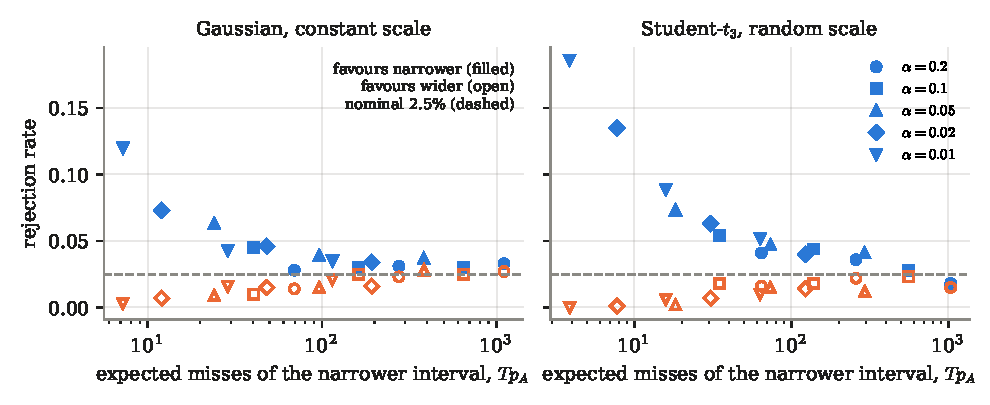
\includegraphics[width=\textwidth]{fig_dm.pdf}
\caption{Rejection rates of the two-sided 5\% Diebold--Mariano test under
equal expected scores, against the expected number of misses of the
narrower interval. Blue: the test declares the narrower forecaster better;
orange: the wider. Marker shapes give $\alpha$; the three points per shape
are $T=250$, $1000$ and $4000$.}
\label{fig:dm}
\end{figure}

\paragraph{Sample size.}
In the second design, outcomes are Gaussian, $B$ is the exact central
interval and $A$ is narrowed or widened by $\eta/z$ with $\eta=1/2$
(Section~\ref{sec:gauss}), so that $A$ is worse. For
$\alpha\in\{0.2,0.1,0.05,0.02,0.01,0.005\}$, 200 replications record the
first round at which the EB lower bound exceeds zero. Because the ranges are
constant, the Hoeffding radius is deterministic, and we report the round at
which it falls below $\Delta$. Detection times are recorded on a geometric grid of about 600
points.\footnote{The reported detection time is the first grid round at
which the lower bound exceeds zero, so it may exceed the exact first
round by at most the spacing of the grid, about 2\%.} Figure~\ref{fig:detection} also shows the
sample size at which a fixed-sample one-sided test at level 2.5\% with
known variance has 80\% power, $(z_{0.975}+z_{0.8})^2\Var(d)/\Delta^2$, and the scale
$H^2/(\alpha\Delta^2)$ of Theorem~\ref{thm:lower}, where $\Delta$ is the
expected interval-score difference ($\Delta_{\IS}$ in that theorem).

The EB and fixed-sample curves are parallel to $H^2/(\alpha\Delta^2)$: the
number of rounds grows like $1/\alpha$. The median number of misses at the
EB detection time is nearly constant, between 191 and 237 for the narrowed
interval and between 126 and 181 for the widened one, from $\alpha=0.2$ to
$\alpha=0.005$. The Hoeffding sequence grows like $1/\alpha^2$: it needs
1.2--1.7 times as many rounds as EB at $\alpha=0.2$ and 50--73 times as many
at $\alpha=0.005$, about $1.4$ to $2.7$ million rounds. Anytime validity
costs EB a factor between 1.6 and 2.6 relative to a fixed-sample test that
knows the variance and is valid only at the planned sample size.

With plentiful misses, as here, the Diebold--Mariano test is reliable: at
the sample size $T_{80}$ at which the known-variance test has 80\% power,
its power is 74--84\% with no wrong-sign rejection, and that of the
bootstrap-$t$ test 68--88\%, against 12--38\% for the tuned sequence
(Appendix~\ref{app:tuned}). Interpolating the power of the tuned sequence
between $T_{80}$, $2T_{80}$ and $4T_{80}$ on a logarithmic scale, it
reaches the power that the Diebold--Mariano test has at $T_{80}$ after
1.9 to 3.3 times as many rounds. This factor is close
to the ratio $\log(2/\delta)/(z_{0.975}^2/2)\approx1.9$
of the exponents of a Chernoff bound and of the normal approximation, which
is the price of a finite-sample guarantee.

\begin{figure}[t]
\centering
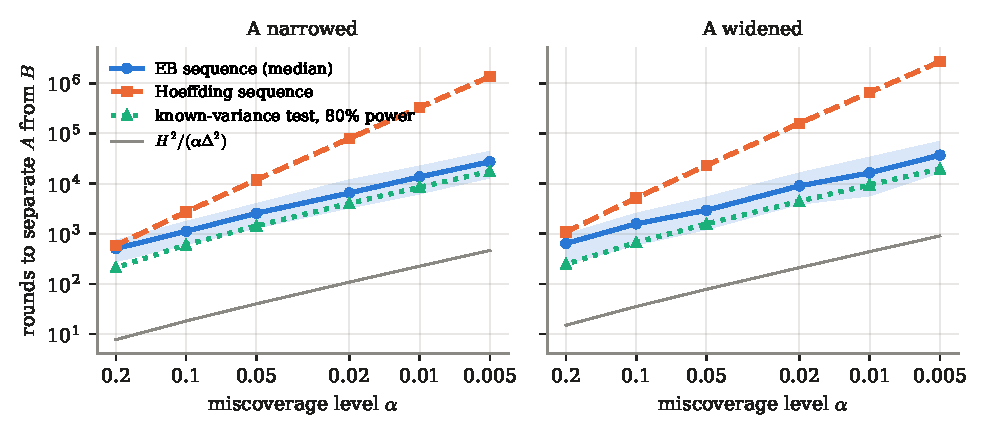
\includegraphics[width=\textwidth]{fig_detection.pdf}
\caption{Rounds needed to separate a narrowed or widened Gaussian interval
from the exact one. EB: median first round at which the 95\% lower bound
exceeds zero, with the 10\%--90\% band over 200 replications. Hoeffding:
round at which its deterministic radius falls below $\Delta$. Known-variance test:
sample size for 80\% power with known variance. Grey: the scale of the lower
bound, without constants.}
\label{fig:detection}
\end{figure}
